\chapter{Results}
\label{results}


\section{Implementation of the Percolator algorithm}
The original Percolator algorithm (version~3.2) finds 5412 cross-linked PSMs with a q-value of $\leq1\%$ on the used dataset~(see Chapter~\ref{lab:matmet:dataset}). The re-implementation in python yields 5450 such PSMs on rank 1.\\\\
The implementation of feature normalization yielded an increase in the number of confident PSMs found, as the curves and legend in Figure~\ref{fig:feature_normalization} show. This type of plot is explained in Section~\ref{lab:results:pseudo_rocs}. The performance of Pycolator with feature normalization is better from the first iteration on, and increases until iterations~7~or~8, when the results converge. Without feature normalization, the area under the pseudo ROC increases until iteration~3, when it begins to oscillate. \\
\renewcommand{\baselinestretch}{0.9}
\begin{figure}
	\normalsize
	\centering
	\begin{subfigure}{0.49\textwidth}
		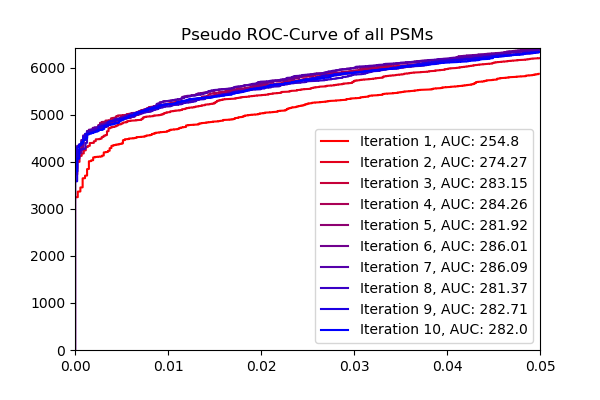
\includegraphics[width = \textwidth]{figures/noNorming.png}
		\caption{}
		\label{fig:before_feature_normalization}
	\end{subfigure}
	\hfill
	\begin{subfigure}{0.49\textwidth}
		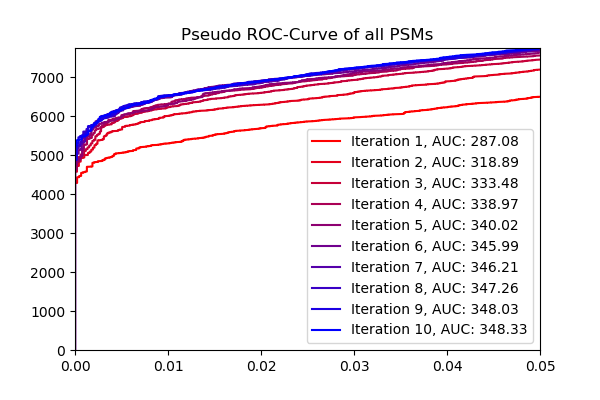
\includegraphics[width = \textwidth]{figures/norming.png}
		\caption{}
		\label{fig:after_feature_normalization}
	\end{subfigure}
	\caption[Results of feature normalization]{Result of Pycolator without~(\ref{fig:before_feature_normalization}) and with~(\ref{fig:after_feature_normalization}) the implementation of feature normalization. }
	\label{fig:feature_normalization}
\end{figure}
\renewcommand{\baselinestretch}{1}

\section{Adapting Percolator to Cross-link Identification}
\label{lab:results:pseudo_rocs}
To evaluate the performance of the model, a method returning pseudo ROCs and their AUC after every iteration and for cross-links, non-cross-links and the whole dataset was implemented. An example of these plots are shown in Figure~\ref{fig:results:pseudo_rocs}. \ref{fig:results:pseudo_rocs_nXL}~shows the pseudo ROC of the non-cross-linked PSMs in every iteration, \ref{fig:results:pseudo_rocs_XL}~the cross-linked and \ref{fig:results:pseudo_rocs_all}~all of the PSMs. In each, every iterations pseudo ROC curve has its own color, fading from red in iteration~1 to blue in iteration~10. The colors can be assigned from the legend, which also shows the area under the depicted pseudo ROC curve. Every curve ranges from q-values~$0$~to~$5\%$ and the y-axis is scaled appropriate for the data. As explained in Subsection~\ref{lab:background:roc}, a steeper and further to the northwest ROC curve represents better classification. Thus, Figure~\ref{fig:results:pseudo_rocs_all} shows that the result of Pycolator improves over most iterations.\\
\renewcommand{\baselinestretch}{0.9}
\begin{figure}
	\normalsize
	\centering
	\begin{subfigure}{0.49\textwidth}
		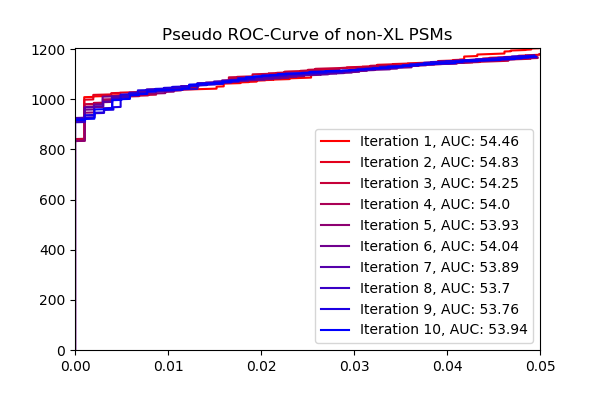
\includegraphics[width = \textwidth]{figures/pseudoROC_non-XL.png}
		\caption{}
		\label{fig:results:pseudo_rocs_nXL}
	\end{subfigure}
	\hfill
	\begin{subfigure}{0.49\textwidth}
		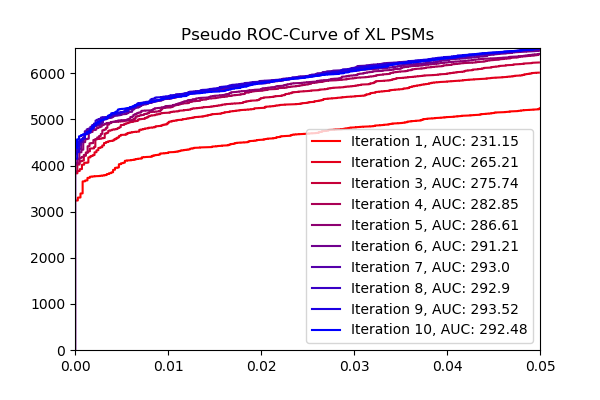
\includegraphics[width = \textwidth]{figures/pseudoROC_XL.png}
		\caption{}
		\label{fig:results:pseudo_rocs_XL}
	\end{subfigure}
	\hfill
	\begin{subfigure}{0.49\textwidth}
		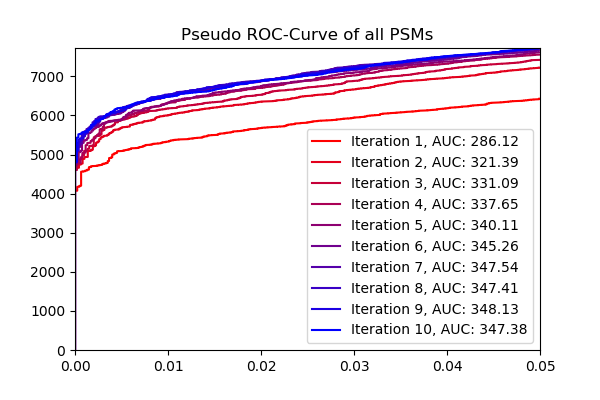
\includegraphics[width = \textwidth]{figures/pseudoROC_all.png}
		\caption{}
		\label{fig:results:pseudo_rocs_all}
	\end{subfigure}
	\caption[Examples of pseudo ROC curves as produced by Pycolator]{Example of the plots output by Pycolator, generated by running with default parameters on the given dataset~(see Chapter~\ref{lab:matmet:dataset}). \ref{fig:results:pseudo_rocs_nXL}~shows the result of non-cross-linked PSMs, \ref{fig:results:pseudo_rocs_XL}~that of cross-linked and~\ref{fig:results:pseudo_rocs_all} that of all PSMs in the dataset.}
	\label{fig:results:pseudo_rocs}
\end{figure}
\renewcommand{\baselinestretch}{1}

\subsection{Different Ranks}
\label{lab:results:ranks}
Figure~\ref{fig:before_optimalranking} shows the pseudo ROCs of Pycolator with and without the optimalRanking feature disabled. \ref{fig:all_ranks} was plotted when Pycolator used all PSMs available, meaning all ranks, and only at the end PSMs ranking lower than~$1$ were excluded. \ref{fig:only_rank_one} is the result of running Pycolator only with rank 1 PSMs of the given dataset~(see Chapter~\ref{lab:matmet:dataset}) and~\ref{fig:optimalranking} shows the final result with the new feature.\\
As one can see, without the new mechanism Pycolator gradually improves the area under the curve and takes $5$ and $4$ iterations to roughly converge when given every PSM or only rank 1 PSMs to train respectively. This can be seen by the AUC results after every iteration or the ROC curves themselves. The end result, however, is better when removing the lower ranking PSMs right at the beginning (AUC of $345.79$) instead of in the end (AUC of $343.21$ after dropping the lower ranking PSMs). Since in the latter case Pycolator ended with an AUC of $343.79$ as one can see in~\ref{fig:all_ranks}, dropping the PSMs slightly worsened the end result. With the new feature, the algorithm takes about $5$ iterations to converge, then performs a jump and again improves over two iterations. The end result, an AUC of $348.13$, is higher than both alternatives. A t-test with the AUC results of $10$~repetitions between the new procedure and providing Pycolator with all PSMs yielded a p-value of $2.77\cdot10^{-12}$ and between the new procedure and providing Pycolator with only rank~one PSMs yielded $4.17\cdot10^{-9}$ as p-value.
\renewcommand{\baselinestretch}{0.9}
\begin{figure}
	\normalsize
	\centering
	\begin{subfigure}{0.49\textwidth}
		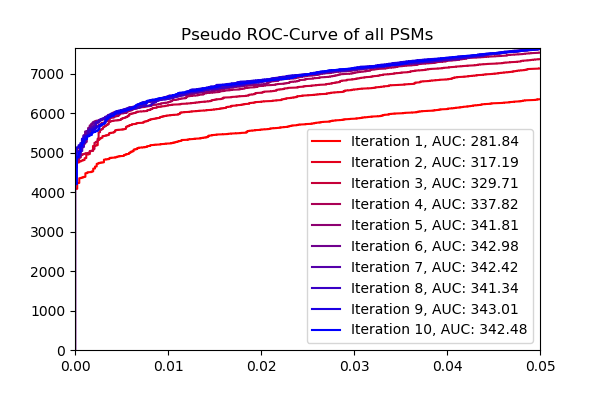
\includegraphics[width = \textwidth]{figures/allRanks.png}
		\caption[Result of dropping lower ranks at the end]{The resulting pseudo ROCs (explained in Section~\ref{lab:results:pseudo_rocs}) if Pycolator is given every PSM regardless of its rank. Lower ranking PSMs are only dropped in the end, which results in a final AUC of $343.21$.}
		\label{fig:all_ranks}
	\end{subfigure}
	\hfill
	\begin{subfigure}{0.49\textwidth}
		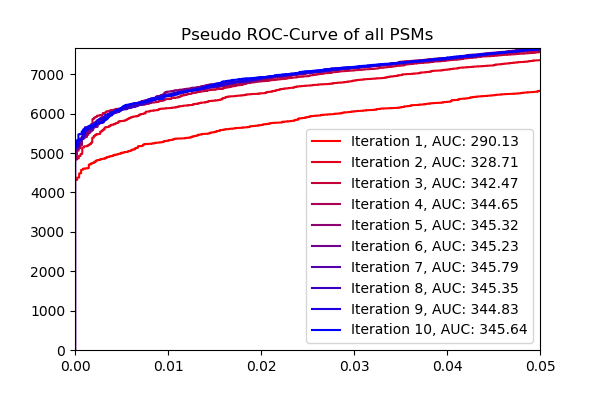
\includegraphics[width = \textwidth]{figures/onlyFirstRank.png}
		\caption[Result of dropping lower ranks at the start]{The resulting pseudo ROCs (explained in Section~\ref{lab:results:pseudo_rocs}) if Pycolator is given only the top scoring peptide for every spectrum. Lower ranking PSMs are dropped before running the algorithm.}
		\label{fig:only_rank_one}
	\end{subfigure}
	\begin{subfigure}{0.75\textwidth}
		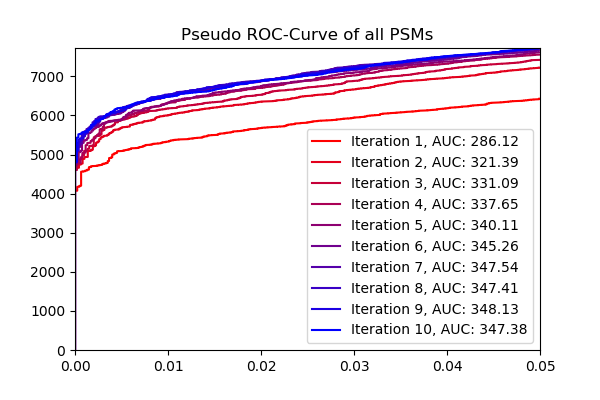
\includegraphics[width = \textwidth]{figures/optimalRanking.png}
		\caption[Result of the new ranking procedure]{The resulting pseudo ROCs (explained in Section~\ref{lab:results:pseudo_rocs}) if Pycolator is run with the newly implemented feature. It first trains with every PSM available, and after the results converge, lower ranking PSMs are dropped. Then, the algorithm runs for some more iterations.}
		\label{fig:optimalranking}
	\end{subfigure}
	\caption[Performance of strategies regarding different ranks]{Results of running Pycolator with different strategies as to how lower ranking PSMs are dealt with.}
	\label{fig:before_optimalranking}
\end{figure}
\renewcommand{\baselinestretch}{1}

\subsection{Characteristics of Cross-linked PSMs}
\subsubsection{a) Proportions of Different Classes}
\label{lab:results:proportions}
Maintaining the proportion of classes works as intended: The log of two test runs of Pycolator when it calculated and output the ratio of targets to decoys in every of the outer split and the whole dataset showed following results: Without maintaining the ratios of target to decoy PSMs in each of the three splits, these ranged from $1.173$ to $1.203$, while the ratio is $1.8865$ in the whole dataset. With maintaining the ratio according to the new method however, these ranged from $1.18862$ to $1.18870$, while the ratio is $1.18865$ in the whole dataset.\\
The evaluation produced the results shown in
%figure~\ref{fig:results:maxminmedian} and
Table~\ref{tab:results:maxminmedian}. The AUC of the best run is lower and the AUC of the worst run is higher for cross-linked and all PSMs when balancing the splits, meaning the variation could be reduced. The AUC of the median run is slightly higher for all categories, for all PSMs by $0.14\%$. 
\renewcommand{\baselinestretch}{0.9}
%\begin{figure}
%	\normalsize
%	\centering
%	\begin{subfigure}{\textwidth}
%		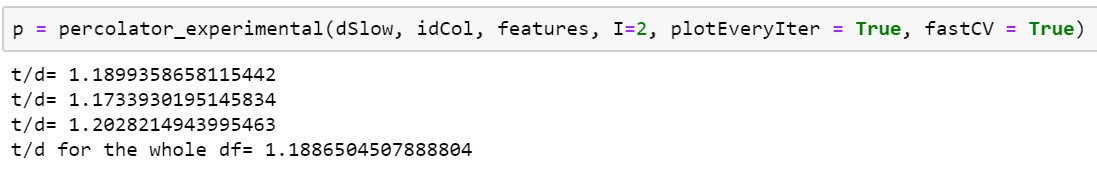
\includegraphics[width = \textwidth]{figures/prop_not_kept_code.jpg}
%		\caption{}
%		\label{fig:results:prop_not_maintained}
%	\end{subfigure}
%	\begin{subfigure}{\textwidth}
%		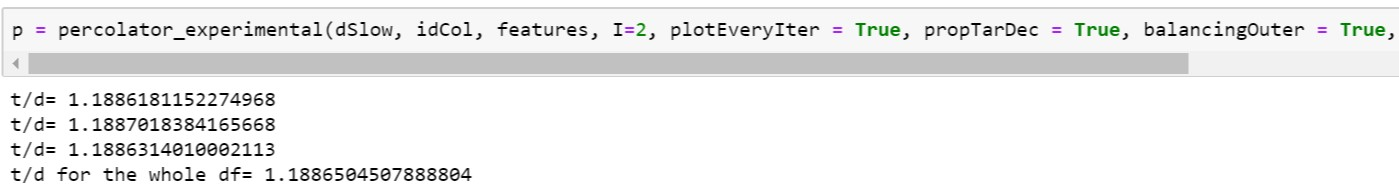
\includegraphics[width = \textwidth]{figures/prop_kept_code.jpg}
%		\caption{}
%		\label{fig:results:prop_maintained}
%	\end{subfigure}
%	\caption[Maintaining proportions works as intended]{}
%	\label{fig:results:prop_code}
%\end{figure}
%\begin{figure}
%	\normalsize
%	\centering
%	\begin{subfigure}{0.49 \textwidth}
%		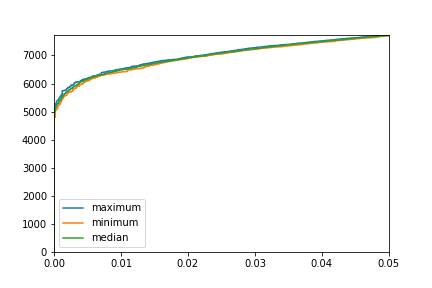
\includegraphics[width = \textwidth]{figures/MaxMinMedian_no_balancing.png}
%		\caption{}
%		\label{fig:results:maxminmedian_not_maintained}
%	\end{subfigure}
%	\hfill
%	\begin{subfigure}{0.49 \textwidth}
%		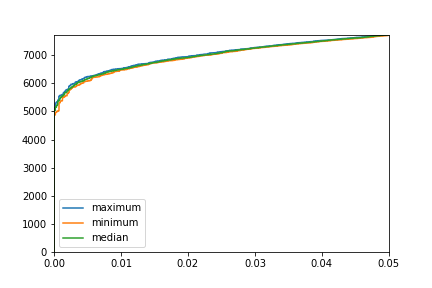
\includegraphics[width = \textwidth]{figures/MaxMinMedian_balancing.png}
%		\caption{}
%		\label{fig:results:maxminmedian_maintained}
%	\end{subfigure}
%	\caption[pseudo ROCs with and without balancing of classes]{Maximum, minimum and median PSMs found at every q-value over each of the 10 sampling rounds. \ref{fig:results:maxminmedian_not_maintained} shows the results without maintaining the proportions, \ref{fig:results:maxminmedian_maintained} with balancing enabled.}
%	\label{fig:results:maxminmedian}
%\end{figure}
\begin{table}[htbp]
	\normalsize
	\centering	
	\caption[Area under the pseudo ROC curves with and without balancing of classes]{Shows the area under the pseudo curves of cross-linked, non-cross-linked and all PSMs in the best, worst and median run w.r.t. the AUC of the pseudo ROC of all PSMs. Pycolator was run with and without balancing of target/decoy and cross-linked/non-cross-linked classes in outer and inner splits 10 times each.}
	\begin{tabular}{r|l||rrr}
		\multicolumn{2}{c}{AUC of pseudo ROC} & maximum & minimum & median \\
		\hline
		\multirow{3}[0]{*}{balancing} & cross-linked & 293.91 & 293.12 & 293.58 \\
		& non-cross-linked & 53.85 & 53.76 & 53.84 \\
		& all PSMs & 348.65 & 347.48 & 348.19 \\
		\hline
		\multirow{3}[0]{*}{no balancing} & cross-linked & 294.42 & 291.51 & 292.86 \\
		& non-cross-linked & 53.63 & 54.34 & 53.78 \\
		& all PSMs & 349.14 & 347.04 & 347.69 \\
	\end{tabular}
	\label{tab:results:maxminmedian}
\end{table}
\renewcommand{\baselinestretch}{1}

\subsubsection{b) Imputation}
\label{lab:results:imputation}
The resulting pseudo ROCs and their AUC for all PSMs are shown in Figure~\ref{fig:results:imputation}. The pseudo ROCs for cross-linked and not cross-linked PSMs show similarly few differences.
\renewcommand{\baselinestretch}{0.9}
\begin{figure}
	\normalsize
	\centering
	\begin{subfigure}{0.49 \textwidth}
		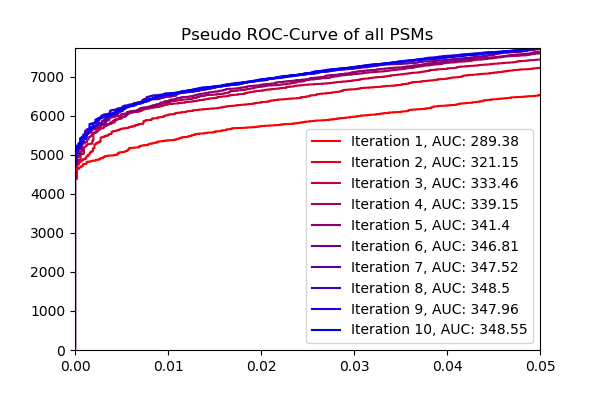
\includegraphics[width = \textwidth]{figures/no_imputation.png}
		\caption{}
		\label{fig:results:imputation_no}
	\end{subfigure}
	\hfill
	\begin{subfigure}{0.49 \textwidth}
		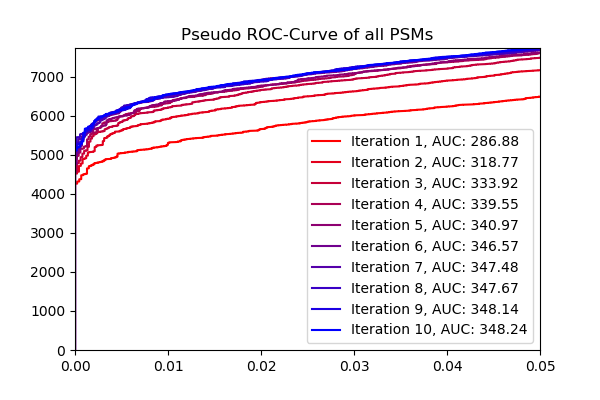
\includegraphics[width = \textwidth]{figures/imputation.png}
		\caption{}
		\label{fig:results:imputation_yes}
	\end{subfigure}
	\caption[Effect of imputation on model performance]{Results of running Pycolator with~(\ref{fig:results:imputation_yes}) and without~(\ref{fig:results:imputation_no}) the use of imputation. Both are very similar.}
	\label{fig:results:imputation}
\end{figure}
\renewcommand{\baselinestretch}{1}

\subsubsection{c) Splitting the Dataset}
\label{lab:results:splitting}
The results of splitting the dataset by cross-linked and non-cross-linked PSMs before running Pycolator are shown in Figure~\ref{fig:results:splitting_xl}. This yielded an AUC of~$350.55$, which is slightly higher than when running Pycolator on all PSMs~(typically $348.5$). Splitting by the cross-linked nucleotide~(results depicted in Figure~\ref{fig:results:splitting_bases}) yielded an AUC of~$389.22$.
\renewcommand{\baselinestretch}{0.9}
\begin{figure}
	\normalsize
	\centering
	\begin{subfigure}{0.49 \textwidth}
		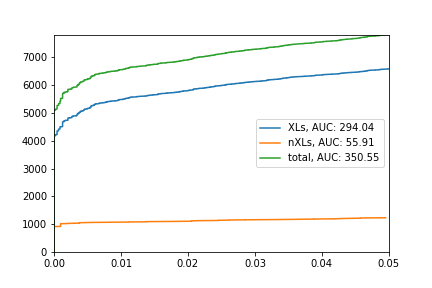
\includegraphics[width = \textwidth]{figures/split_by_xl.png}
		\caption{}
		\label{fig:results:splitting_xl}
	\end{subfigure}
	\hfill
	\begin{subfigure}{0.49 \textwidth}
		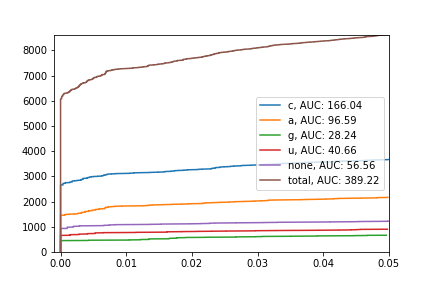
\includegraphics[width = \textwidth]{figures/split_by_bases.png}
		\caption{}
		\label{fig:results:splitting_bases}
	\end{subfigure}
	\caption[Model performance after splitting the dataset]{Resulting pseudo ROCs and their AUC for each split and the combined dataset when splitting the dataset by \ref{fig:results:splitting_xl})~cross-linked and non-cross-linked PSMs, \ref{fig:results:splitting_bases})~the cross-linked nucleotide. XLs stands for cross-linked PSMs and nXLs for non-cross-linked PSMs.}
	\label{fig:results:splitting}
\end{figure}
\renewcommand{\baselinestretch}{1}

\subsection{Small datasets}
\label{lab:results:small_datasets}
When measuring the AUC in the first experiment, a roughly linear correlation to the datasets size was found. However, the AUC could not be measured when the dataset became smaller than approximately $200$ PSMs, as shown in Figure~\ref{fig:results:small_dataset_first_auc}. The number of PSMs at $1\%$ FDR was larger relative to dataset size when using a smaller portion of the dataset, whether using a fixed~(\ref{fig:results:small_dataset_first_ratio_dxl}) or Pycolator's score~(\ref{fig:results:small_dataset_first_auc_ratio_pxl}). In the case of Pycolator, with smaller dataset size also more fluctuations occurred.\\
The second experiment yielded following results: Figure~\ref{fig:results:small_dataset_snd_expected} shows the portion of the dataset that was originally estimated to have a q-value of $<1\%$. The ratio of how many PSMs were assigned such a q-value after the sampling to before, is shown in Figure~\ref{fig:results:small_dataset_snd_found_dxl} without re-calculating the score with Pycolator. Figure~\ref{fig:results:small_dataset_snd_comparison} shows how well the Pycolator~score performed compared with the precomputed NuXL-score when measured by the identifications with $1\%$ q-value or area under the pseudo ROC curve. The boxplots for the smallest datasets do not always contain 10 results, because Pycolator did, depending on the split, not work on datasets with $12$ to $93$ PSMs.\\
\renewcommand{\baselinestretch}{0.9}
\begin{figure}
	\normalsize
	\centering
	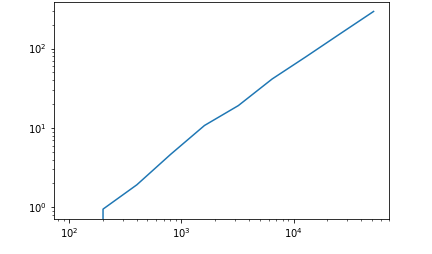
\includegraphics[width = 0.49\textwidth]{figures/aucs_perc.png}
	\caption[Correlation between AUC and dataset size]{The AUC of a Pycolator run on the y-axis is plotted against the size of the dataset sampled as described in Subsection~\ref{lab:matmet:small_datasets} on the x-axis. Below about 200 PSMs in the dataset, the pseudo ROC consisted of data at one q-value and thus enclosed an area of 0 or could not be determined.}
	\label{fig:results:small_dataset_first_auc}
\end{figure}
\begin{figure}
	\normalsize
	\centering
	\begin{subfigure}{0.49 \textwidth}
		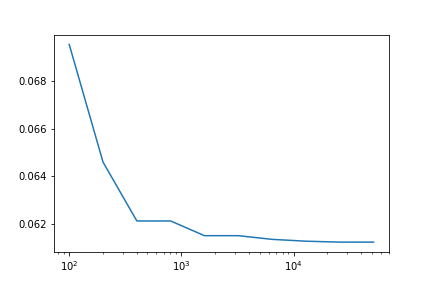
\includegraphics[width = \textwidth]{figures/ratio_idents_whole_df_NuXL.png}
		\caption{}
		\label{fig:results:small_dataset_first_ratio_dxl}
	\end{subfigure}
	\hfill
	\begin{subfigure}{0.49 \textwidth}
		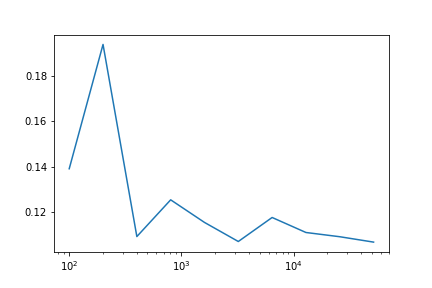
\includegraphics[width = \textwidth]{figures/ratio_idents_whole_df_percolator.png}
		\caption{}
		\label{fig:results:small_dataset_first_auc_ratio_pxl}
	\end{subfigure}
	\caption[Portion of high-confidence PSMs in different dataset sizes]{The portion of PSMs in the sampled dataset with an estimated FDR of $1\%$ on the y-axis is plotted against the datasets size on the x-axis. Left~(\ref{fig:results:small_dataset_first_ratio_dxl}) when estimating the FDR based on the unchanged NuXL-score, and right~(\ref{fig:results:small_dataset_first_auc_ratio_pxl}) after running Pycolator on the sampled dataset.}
	\label{fig:results:small_dataset_first_auc_ratio}
\end{figure}
\begin{figure}
	\normalsize
	\centering
	
\end{figure}
\begin{figure}
	\normalsize
	\centering	
	\begin{subfigure}{0.49 \textwidth}
		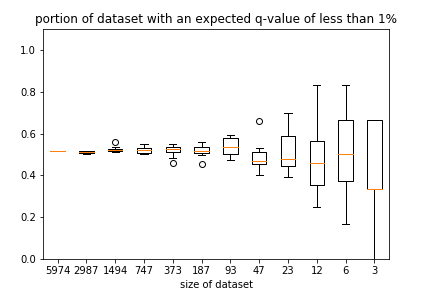
\includegraphics[width = \textwidth]{figures/expected.png}
		\caption[Portion of the dataset with high-confidence PSMs]{.}
		\label{fig:results:small_dataset_snd_expected}
	\end{subfigure}
	\hfill
	\begin{subfigure}{0.49 \textwidth}
		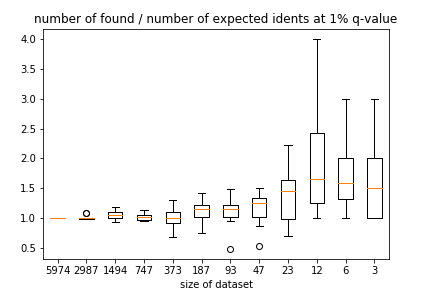
\includegraphics[width = \textwidth]{figures/found_vs_expected_dxl.png}
		\caption{}
		\label{fig:results:small_dataset_snd_found_dxl}
	\end{subfigure}
	\caption[Effect of splitting on dataset and FDR estimation]{a) Proportion of high confidence PSMs~(q-value $\leq1\%$) in the subsampled dataset from all PSMs with $10\%$ FDR is plotted on the y-axis. b) The ratio of high confidence PSMs found after to before re-calculating the FDR in the sampled dataset is plotted. In both cases, the x-axis shows the datasets size, and the data from every of the 10 repetitions is shown combined in a boxplot.}
	\label{fig:results:small_dataset_snd_found}
\end{figure}
\begin{figure}
	\normalsize
	\centering
	\begin{subfigure}{0.49 \textwidth}
		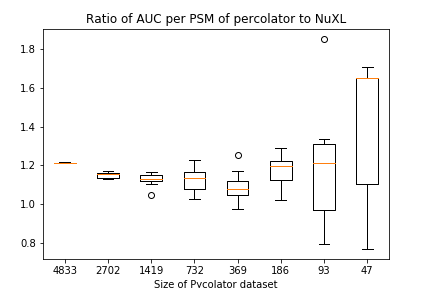
\includegraphics[width = \textwidth]{figures/auc_p_vs_ori.png}
		\caption{}
		\label{fig:results:small_dataset_snd_comparison_auc}
	\end{subfigure}
	\hfill
	\begin{subfigure}{0.49 \textwidth}
		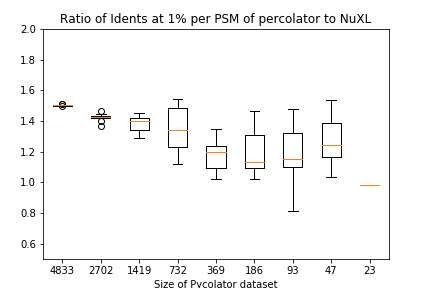
\includegraphics[width = \textwidth]{figures/idents_p_vs_ori_zoomed.png}
		\caption{}
		\label{fig:results:small_dataset_snd_comparison_idents}
	\end{subfigure}
	\caption[Performance of Pycolator on smaller datasets]{The ratio of Pycolators performance to the unchanged NuXL-score on the y-axis is plotted against the datasets size on the x-axis. Left~(a), to measure the performance, the area enclosed by the pseudo ROC is used, right~(b) the number of PSMs with a q-value of~$\leq1\%$. The data from every of the 10 repetitions is shown combined in a boxplot. While the median performance ratio measured by the AUC increases for datasets smaller than about $200$ PSMs, Pycolator identifies less PSMs with a confidence of $1\%$ the smaller the dataset is.}
	\label{fig:results:small_dataset_snd_comparison}
\end{figure}
\renewcommand{\baselinestretch}{1}
	